\documentclass{article}
\usepackage[utf8]{inputenc}
\usepackage{graphicx}
\usepackage{float} 
\usepackage{array}
\textheight 24cm
\textwidth 16cm
\oddsidemargin 0cm
\evensidemargin 0cm
\topmargin 0cm
\hoffset -0mm
\voffset -20mm
\usepackage[]{listings}
\usepackage{amsmath}
\title{Geometric Modeling}
\author{Manuel Camargo & Mohamed Traoré &  Nicolas Gindrier}
\date{}
\begin{document}

\maketitle
\section*{Summary and presentation}
\begin{figure}[H]
   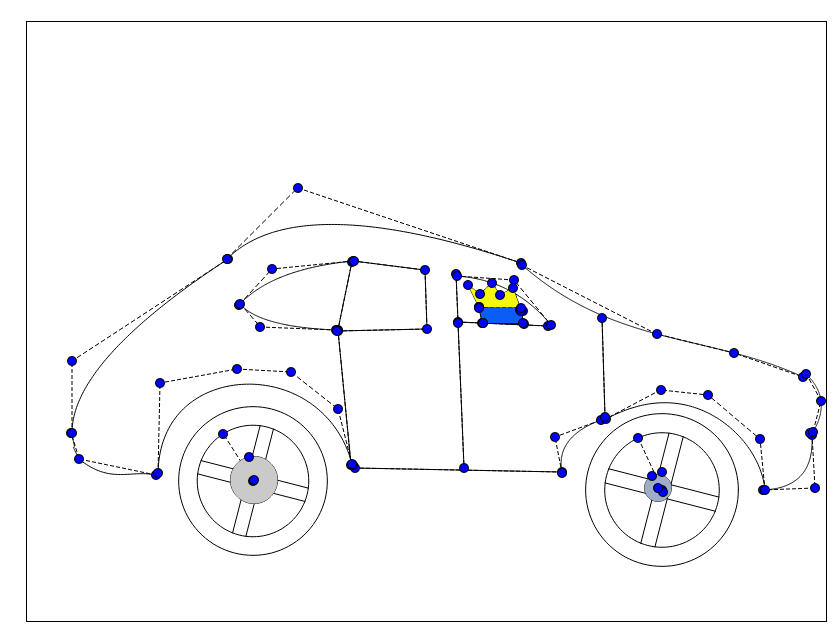
\includegraphics[scale = 0.5]{Pictures/narutovoiture.png}
\end{figure}
\section*{Organization}
We used Github. Manuel worked on parameterizations of 2D curves (Aiken Centripetal/Chordal), 1D curves and delCurve. Mohamed made 1D curves (sinus) and 2D curves (Lagrange/smooth) and Nicolas did essentially 2D curves (Hermite1-closed, Bezier and Gear, Wheel, even if there are not curves). 
\section*{Curves}
\subsection*{Curves 1-D}
\subsubsection*{Sinusoidal}
The idea comes from the fact that the function $t \longmapsto t+\sin t$ has an interessing form as shown
on the following figure. It will help us to do some kinds of movement.
\begin{figure}[H]
	\center
   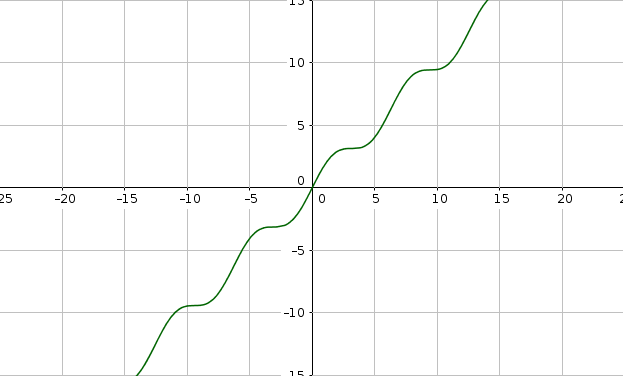
\includegraphics[scale = 0.35]{Pictures/sin1.png}
\end{figure}
Now, the goal is to find a function like the previous sinusoidal function which connects two given points
$A(t_A;x_A)$ and $B(t_B;x_B)$.
And after looking for it, we find the function defined by :
\[
	t \longmapsto x_A + (x_B-x_A)\frac{t-t_A}{t_B-t_A} + \Delta\sin(\Omega(t-t_A))\sin(\Omega(t_B-t))
\]
Where $\Delta$ is the amplitude and $\Omega$ is the pulsation in terms of signal.\\
This function is a sinusoidal function and we can also remark that $f(t_A)=x_A$ and $f(t_B)=x_B$.
\subsection*{Curves 2-D}
\subsubsection*{Bezier-Aitken}
These both curves are coded from the same way. A recursive function on the contrrol points is called. We store points in a static tab and we linked these points after. It is also used for \textit{Hermite1} and \textit{Hermiteclosed}. For \textit{Aitken} we use a uniform parameterization. 
\begin{figure}[H]
   \includegraphics[scale = 0.3]{Pictures/bezier-aitken.png}
\end{figure}
\subsubsection*{Hermite1-Hermite closed}
These curves are made with some Hermite cubic splines, based on P1, P2 and their tangent. That allows to have $C^1$ closed curves. The difficulty is to impose good direction, weight and sense for tangents.\\ 
The general formula is :
\begin{equation}
  \left\{
  \begin{aligned}
    D_{xi} = l L_1 + m L_2\\
    D_{yi} = l L_1 \dfrac{Y_{i+1} - Y_{i}}{X_{i+1} - X_{i}} + m L_2 \dfrac{Y_{i} - Y_{i-1}}{X_{i} - X_{i-1}}\\
  \end{aligned}
  \right.
\end{equation}
We adapt it for the first and the last point. Moreover $\dfrac{Y_{i+1} - Y_{i}}{X_{i+1} - X_{i}}$ is bounded.\\
l and m are equal to 1 or -1 according to tests of the form $X_{i+1} - X_{i}$, that changes the sense of the curve.\\
$L_1$ and $L_2$ are the weight of derivatives, they are a projection. Actually this is a weighted average. \\
\begin{figure}[H]
   \includegraphics[scale = 0.5]{Pictures/rapport2.png}
\end{figure}

\begin{figure}[H]
   \includegraphics[scale = 0.5]{Pictures/hermite.png}
\end{figure}
\subsubsection*{Wheel-Gear}
It is not really curves. The goal here is to play with the variable \textit{frame}. We are midway between cartoon and CAD.\\
In both cases \textit{frame} is traduced as rotation speed. \\
For \textit{Wheel} we draw two circles. We use the points of the little circle in scrolling the array according to \textit{frame}. To draw a radius we link a point of the array at the size(array)/2 point. In playing with that and modulo we can draw a rolling wheel.
For gear we implicitely use a rotation matrix. We have three angles (see scheme) : $\alpha$, to draw the gear, $\beta$, to make rolling the gear, depending on frame and an angle depending on the mouse position (it is for follow the mouse and engage another gear, the absolute value of this angle is $2\ arccos(d(\dfrac{mouse,center}{2 R}))$These three angles are added. $\beta$ is computed such that the angular speed of whatever gear be the same ($\beta$ is inversely proportional to the radius).\\ )
Actually there is a repetition of 4 points, at every rotation we choose to add or substract at the radius the half-size of a teeth. Besides, the radius is computed to have an whole number of teeth.\\
\begin{figure}[H]
   \includegraphics[scale = 0.5]{Pictures/rapport1.png}
\end{figure}
So the user can drow a gear in clicking one or two times to chose the sense of rotation (an odd number for clockwise, otherwise counter-clockwise) then right-click for the radius (in fact almost the radius as above explained).
\begin{figure}[H]
   \includegraphics[scale = 0.3]{Pictures/gear-wheel.png}
\end{figure}
\subsection*{Lagrange interpolation}
The aim of this part is to find a polynomial function with degree $n$ that interpolates $(n+1)$ 
different given points. By using Lagrange method, the polynomial function that we are looking for is defined by :
\[ 
	L(x) = \sum_{i=0}^{n}y_i \left(\prod_{\substack{j=0 \\ j\ne i}}^{n}\frac{x-x_j}{x_i-x_j}\right)
\]
where $(x_i;y_i)$ are the coordinates of the $i^{\text{th}}$ point.\\
We can see an exemple of Lagrange interpolation on the figure below. 
\begin{figure}[H]
	\center
   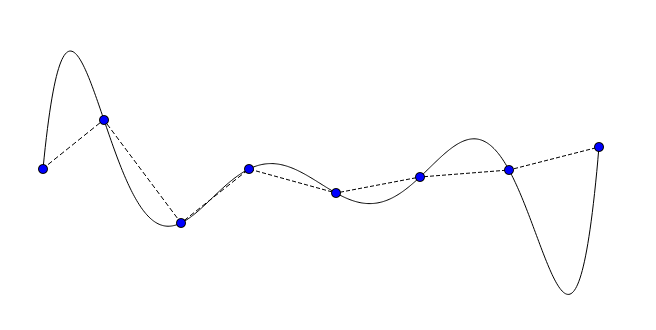
\includegraphics[scale = 0.35]{Pictures/lag1.png}
\end{figure}
\subsection*{Least square approximation}
In this part we have to find a polynomial curve of degree $p$ that approximates $(n+1)$ given points.
We know that if $p=n$, we are in the case of parametrical interpolation which is done by \textit{Aitken}
method. So we will suppose that $p<n$.  \\
Let $\displaystyle A(x) = \sum \limits_{i=0}^{p}a_ix^i$ be the polynomial curve of degree $p$ that we need.
 \begin{align*}
 	\forall \ 0 \le q \le n, A(x_q) = y_q+\epsilon_q 
 	&\iff
 	\left\{
 	\begin{array}{c c c}
 		A(x_0) &=& y_0 + \epsilon_0 \\
 		\vdots &\vdots& \vdots  \\
 		A(x_j) &=& y_j + \epsilon_j \\
 		\vdots &\vdots& \vdots  \\
 		A(x_n) &=& y_n + \epsilon_n
 	\end{array}
 	\right.
 	\iff
 	\left\{
 		\begin{array}{c c c}
 		\sum \limits_{i=0}^{p}a_ix_0^i &=& y_0 + \epsilon_0 \\
 		 \vdots &\vdots& \vdots  \\
 		\sum \limits_{i=0}^{p}a_ix_j^i &=& y_j + \epsilon_j \\
 		\vdots &\vdots& \vdots \\
 		\sum \limits_{i=0}^{p}a_ix_n^i &=& y_n + \epsilon_n
 		\end{array}
 	\right.\\
 	&\iff 
 	\begin{pmatrix}
 		1   & \cdots & x_0^j &  \cdots & x_0^p \\  
 	 \vdots & \cdots & \cdots &  \cdots & \cdots \\
 		1 & \cdots & x_k^j &  \cdots & x_k^p \\
 	 \vdots & \cdots & \cdots &  \cdots & \cdots \\ 		
 		1 & \cdots & x_n^j &  \cdots & x_n^p 
 	\end{pmatrix}
 	\begin{pmatrix}
 		a_0 \\
 		\vdots \\
 		a_j \\
 		\vdots \\
 		a_p
 	\end{pmatrix} =
 	 	\begin{pmatrix}
 		y_0 \\
 		\vdots \\
 		y_k \\
 		\vdots \\
 		y_n
 	\end{pmatrix}+
 	 	\begin{pmatrix}
 		\epsilon_0 \\
 		\vdots \\
 		\epsilon_k \\
 		\vdots \\
 		\epsilon_n
 	\end{pmatrix} \\
 	&\iff Au = y + \epsilon
 \end{align*}
 Now, we want to minimize the euclidean norm of errors $\epsilon$ that is to say find $u^*$ such that
 \[  
 	u^* = \min_{u} \Vert \epsilon \Vert^2 = \min_{u} \Vert Au - y \Vert^2
 \]
 We also need an important result which is : 
 \[ \,(^tAA)u = \,^tAy \iff u =  (^tAA)^{-1}\,(^tAy)\] 
 The following figure is the approximation of $10$ points by a polynomial of degree $8$ using
 least square method.
 \begin{figure}[H]
	\center
   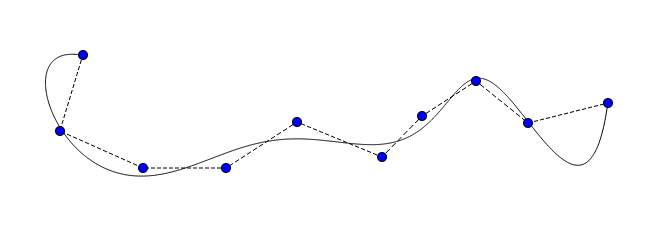
\includegraphics[scale = 0.4]{Pictures/sq1.png}
\end{figure}
\subsection*{others} %for example DelCurve
\section*{Prospects}
We had a lot of ideas but some of them have not been made. It was because of time, or because we fear to modify some files. We do not master the architecture of the whole project. For example matstering scene.h would allowed many things, like to save. 
\end{document}
